\documentclass{homework}
% \usepackage{graphicx} % Required for inserting images
\usepackage{amsmath}
\usepackage{gensymb}
\usepackage{subfig}
\usepackage{float}

\class{ECEN 5738}
\title{Homework 5}
\author{Sean Jennings}
\date{April 8, 2024}

\begin{document}
\maketitle

\section{Problem 1}

To show each non-autonomous system has an asymptotically stable equilibrium
at the origin, we find a time-varying Lyapunov function
$V: [0, \infty) \times D \to \R$ which over some domain $D \subset \R^n$ satifies:
\begin{enumerate}
    \item $W_1(x) \leq V(t, x) \leq W_2(x)$
    \item $\dot{V}(t, x) = \frac{\delta V}{\delta t} +
        \frac{\delta V}{\delta x}f(t, x) \leq -W(x)$
\end{enumerate}
for some continuous positive definite functions $W_1$, $W_2$, and $W_3$.

\begin{letterenum}
\item Try $V(t, x) = 1/2 \cdot x^T x$. This is clearly positive definite,
and thus bounded by positive definite time-invariant functions.
We check that the derivative is negative definite: taking the derivative
yields:
\begin{align*}
    \dot{V}(t, x) = x^T \dot{x} &= x^T \biggl( -x + \norm{x}^2 \mat{g(t) \\ h(t)}\biggr) \\
        &= - x^T x + \norm{x}^2 x^T \mat{g(t) \\ h(t)} \\
        &= - \norm{x}^2 \biggl( 1 - x^T \mat{g(t) \\ h(t)}\biggr) \\
\end{align*}
So $\dot{V}$ is negative definite when $\mat{g(t) & h(t)} x < 1$. Since the
inner product can be bounded by:
\begin{equation*}
    x^T \mat{g(t) \\ h(t)} \leq \normtwo{x}
        \biggl\lVert\mat{g(t) \\ h(t)}\biggr\rVert_2 \leq \sqrt{2} \normtwo{x}
\end{equation*}
$\dot{V}$ is negative definite whenever $\normtwo{x} \leq \sqrt{2}$. Thus, the origin
is asymptotically stable.

\item Let $A$ be the given matrix:
\begin{equation*}
    A := \mat{
        -2 & g(t) \\
        g(t) & -4
    }
\end{equation*}
Try the Lyapunov function $V(t, x) = 1/2 x^T x$. The derivative is given by:
\begin{align*}
    \dot{V}(t, x) &= 1/2 (x^T \dot{x} + \dot{x}^T x) \\
        &= 1/2 ( x^T A(t)x + x^T A(t)^T x) \\
        &= 1/2 x^T (A(t) + A(t)^T) x \\
        &= x^T A(t) x
\end{align*}
where the last equality is due to the fact that $A$ is symmetric.

A general 2x2 matrix $B\in\R^{2\times 2}$ given by
\begin{equation*}
    B = \mat{
        a & b \\
        c & d
    }
\end{equation*}
has characteristic equation
\begin{align*}
    \det{\lambda I - A} &= (\lambda - a) (\lambda - d) - bc \\
        &= \lambda^2 - (a + d) \lambda + (ad - bc) \\
        &= \lambda^2 -\text{Tr}(A) + \det{A}
\end{align*}
Since its eigenvalues are given by
\begin{equation*}
    \lambda_{1,2} = 1/2(\text{Tr}(A) \pm \sqrt{\text{Tr}(A)^2 - 4 \det(A)})
\end{equation*}
we can see the eigenvalues are strictly negative when Tr$(A) < 0$ and $\det(A) > 0$.
Since Tr$(A) = -6$ and $\det{A} = 8 - g(t)^2 \geq 7$, the eigenvalues of $A$
are strictly negative, $A$ is negative definite, and the function $\dot{V}$ is also
negative definite.

\item Let $A$ be the matrix
\begin{equation*}
    A = \mat{-1 & 1 \\ -1 & 0 }
\end{equation*}
The inequality
\begin{align*}
    h(t) x^T A x &=
        h(t) \mat{x_1 \\ x_2}^T A \mat{x_1 \\ x_2} \\
        &= h(t) \mat{x_1 \\ x_2}^T \mat{-x_1 + x_2 \\ -x_1} \\
        &= h(t) (-x_1^2 + x_1 x_2 - x_1 x_2) = -h(t) x_1^2 \\
        &\leq 0
\end{align*}
is due to the fact that $h(t) \geq 0$, and is used below.

Try $V(t, x) = 1/2 x^T x$ as a Lyapunov candidate. Then,
\begin{align*}
    \dot{V}(t, x) &= x^T \dot{x} \\
        &= x^T (h(t) Ax - g(t) \mat{x_1^3 \\ x_2^3}) \\
        &= h(t) x^T A x - g(t) (x_1^4 + x_2^4) \\
        &\leq -g(t) (x_1^4 + x_2^4) \\
        &\leq -(x_1^4 + x_2^4) \\
\end{align*}
shows that $\dot{V}$ is negative definite, and thus the origin is
asymptotically stable.

\end{letterenum}

\section{Problem 2}
\begin{enumerate}[(a)]
\item A continuous function $\alpha: [0, \infty) \to [0, \infty)$ is a
class-$\mathcal{K}$ function if $\alpha(0) = 0$ and $\alpha(r_2) > \alpha(r_1)$
whenever $r_2 > r_1$. $\alpha$ is class-$\mathcal{K}_\infty$ if additional
$\lim_{r\to\infty} \alpha(r) = \infty$.

A continuous function $\beta: [0, \infty) \times [0, \infty) \to [0, \infty)$
is class-$\mathcal{K}\mathcal{L}$ if
\begin{enumerate}[(1)]
    \item for each fixed $t$, $\beta(\cdot, t)$ is class-$\mathcal{K}$, and
    \item for each fixed $r$, $\beta(r, \cdot)$ is strictly decreasing and
        $\beta(r, t) \to 0$ as $t \to \infty$.
\end{enumerate}

\item Before showing that the given function is class $\mathcal{K}\mathcal{L}$,
we will note that the composition $\alpha_1 \circ \alpha_2$ of any class-$\mathcal{K}$
functions $\alpha_1$ and $\alpha_2$ is also class-$\mathcal{K}$, since
\begin{enumerate}[(1)]
    \item the composition of two continuous functions is continuous,
    \item the composition of strictly increasing functions is strictly increasing, and
    \item $\alpha_1(0) = 0$ and $\alpha_2(0) = 0$ implies that
    \begin{equation*}
        (\alpha_1 \circ \alpha_2)(0) = \alpha_1(\alpha_2(0)) = \alpha_1(0) = 0
    \end{equation*}
\end{enumerate}

Now, let $\gamma(r, t) = \alpha_1(\beta(\alpha_2(\cdot), \cdot))$.

Fix $t>0$. Since $\beta(\cdot, t)$ is class-$\mathcal{K}$,
$\gamma(\cdot, t) = \alpha_1 \circ \beta(\cdot, t) \circ \alpha_2$ also is.

Fix $r>0$ and $0 < t_1 < t_2$. Then, since $\beta$ is class-$\mathcal{K}\mathcal{L}$
\begin{equation*}
    s_1 := \beta(\alpha_1(r), t_1) > \beta(\alpha_2(r), t_2) =: s_2.
\end{equation*}
($:=$ and $=:$ indicate symbol definition.)

Thus, since $\alpha_1$ is class-$\mathcal{K}$
\begin{equation*}
    \gamma(r, t_1) = \alpha_1(s_1) > \alpha_1(s_2) = \gamma(r, t_2)
\end{equation*}
and $\gamma$ is strictly decreasing.

Finally, since for any $r > 0$, $\beta(r, t) \to 0$ as $t \to \infty$, we have
\begin{equation*}
    \lim_{t \to \infty} \gamma(r, t) = \lim_{t \to \infty} \alpha(\beta(\alpha_2(r), t))
        = \alpha_1(0) = 0
\end{equation*}

\item For the given $\alpha_1$, $\alpha_2$, and $\beta$, we have
\begin{align*}
    \beta(\alpha_2(r), t) &= r^p e^{-\lambda t} \\
    \gamma(r, t) &= (r^p e^{-\lambda t})^{1/p} \\ &= r e^{\lambda t / p}
\end{align*}


\end{enumerate}

\section{Problem 3}
\begin{letterenum}
\item We look for a time-varying Lyapunov candidate $V: [0, \infty) \times \R^n \to \R$ such that:
\begin{enumerate}
    \item $V(t, x)$ is bounded above and below by a time-invariant positive definite functions of $x$
    \item $\dot{V}(t, x)$ is negative definite, whenever $\norm{x} \geq \rho(\norm{u})$
        for some class-$\K$ function $\rho$.
\end{enumerate}

\begin{equation*}
    V = 1/2 (x_1^2 + x_2^2)
\end{equation*}

We check for negative definiteness of the derivative:
\begin{align*}
    \dot{V} &= x_1 \dot{x}_1 + x_2 \dot{x}_2 \\
        &= x_1 ( -x_1 + x_1^2 x_2) + x_2 (-x_1^3 - x_2 + u) \\
        &= -x_1^2 + x_1^3 x_2 - x_1^3 x_2 - x_2^2 + x_2 u \\
        &= -x_1^2 - x_2^2 + x_2 u
\end{align*}

By Young's inequality, we have
\begin{equation*}
    x_2 u \leq 1/2 x_2^2 + 1/2 u^2
\end{equation*}
So that $\dot{V}$ can be upper bounded by
\begin{align*}
    \dot{V} &\leq -x_1^2 - 1/2 x_2^2 + 1/2 u^2 \\
        &\leq -3/4 x_1^2 - 1/4 x_2 \\
        &\leq -1/4 \norm{x}^2
\end{align*}
whenever
\begin{equation}
    \norm{x} \geq \rho(\norm{u}) := 2 \norm{u}^2
    \label{eq:state-input-ineq}
\end{equation}

since (\ref{eq:state-input-ineq}) implies
\begin{equation*}
    1/2 u^2 - 1/4 x_1^2 - 1/4x_2^2 \leq 0
\end{equation*}

\item By definition of input-state stability (ISS), we have
\begin{equation*}
    \norm{x(t)} \leq \beta(\norm{x(t_0)}, t - t_0) +
        \gamma \biggl( \sup_{t_0 \leq \tau \leq t} \norm{u}\biggr)
\end{equation*}

for some class-$\KL$ function $\beta$ and class-$\K$ function $\gamma$.
So if the system is ISS, the unforced system $\dot{x} = f(x, 0)$ is bounded
by $\beta(\norm{x(t_0)}, t - t_0)$ and therefore is globally asymptotically stable.
The contrapositive also holds: if the unforced system is unstable, the system is
not ISS.

We show the given system is unstable by linearization about the origin.
The unforced linearized system is given by
\begin{equation*}
    \dot{x} = \mat{
        -1 & 1 \\
        1 & 0
    } x =: Ax.
\end{equation*}
We see the eigenvalues of this matrix are
\begin{equation*}
    \lambda_{1,2} = 1/2 (-1 \pm \sqrt{5})
\end{equation*}
and therefore the origin of the non-linear system is an unstable equilibrium.
This shows the system is not ISS.

\item We show the system is not ISS by finding a bounded input $u$ for which
the state grows unbounded. Take $u$ to be constant over time with $u > 1$,
e.g. $u(t) = 2 \forall t \geq0$. Since
\begin{equation*}
    -\text{sat}(x) \geq -1
\end{equation*}
we have
\begin{equation*}
    \dot{x} = -\text{sat}(x) + u \geq 1
\end{equation*}

The solution of the system $x(t)$ is lower bounded by $t + x(0)$,
which approaches infinity as $t \to \infty$. Thus, we have an unbounded 
solution for a bounded input, and the system is not ISS.

\end{letterenum}

\section{Problem 4}
We rewrite the system as the interconnection between two identical 1-dimensional
systems defined by the state dynamics:
\begin{equation*}
    \dot{x} = f(x, u) := -x^3 + u
\end{equation*}

This interconnection is displayed graphically below.

\begin{center}
    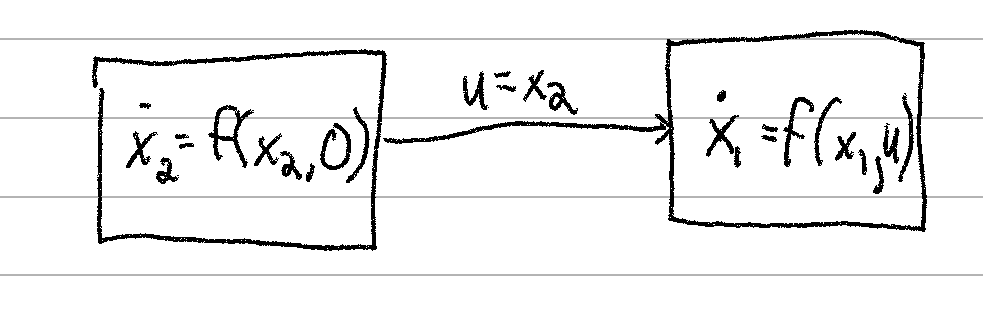
\includegraphics[width=0.5\linewidth]{Images/interconnection.png}
\end{center}

In lecture, we proved two facts:
\begin{enumerate}
    \item The system
    \begin{equation*}
        \dot{x} = -x^r + x^s u
    \end{equation*}
    is ISS if $r$ is an odd integer and $s$ is a real number with $r > s > -1$, and

    \item the series interconnection of ISS systems is globally asymptotically stable.
\end{enumerate}

Taking $r = 3$ and $s=0$, we see that the subsystems in question are both ISS by (1),
and the origin is globally asymptotically by (2).






\end{document}
